\graphicspath{{Images/}}

\section{Úvod}
    \subsection{O projektu}

    \begin{spacing}{1.5}
    \fontsize{14}{14}\selectfont
    
    Cílem projektu je navrhnout a implementovat vestavenou aplikaci v jazyce C pro Wemos D1 R32 w/ ESP32, která bude měřit vzdálenost nejbližšího objektu od senzoru a její hodnotu (v centimetrech) bude zobrazovat na displeji. Kromě toho obsahuje vybavení napájivé pole, senzor VL53L0X pro měření vzdálenosti, OLED displej (IIC), enkoder a sadu propojovacích  vodíčů. 
    \end{spacing}

    \subsection{Zapojení}

    \begin{figure}[h]
        \centering
        \subfigure{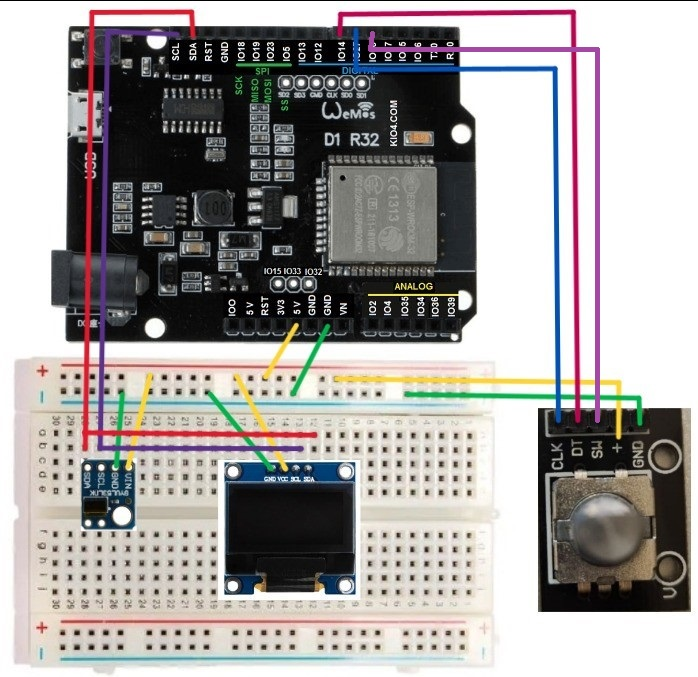
\includegraphics[scale=0.6]{img/schema_zapojeni.jpg}}
        \caption{Schéma zapojení}
        \label{zapojeni}
    \end{figure}
    
    \begin{spacing}{1.5}
        \subsection*{Senzor VL53L0X a OLED Displej}
        \fontsize{14}{14}\selectfont
        \begin{itemize}
        \item VIN senzoru a VCC displeje jsou připojený na \textbf{PLUS} a napojený na pin 5V ESP32
        \item GND senzoru a displeje jsou připojený na \textbf{MINUS} a napojený na pin GND ESP32
        \item SCL displeje je připojený na SCL senzoru a jsou spolu přimo zapojený na pin SCL ESP32  
        \item SDA displeje je připojený na SDA senzoru a jsou spolu přimo zapojený na pin SDA ESP32
        \end{itemize}
    \end{spacing}

    \begin{spacing}{1.5}
        \subsection*{Enkoder}
        \fontsize{14}{14}\selectfont
        \begin{itemize}
        \item VCC je připojený na \textbf{PLUS} a napojený na pin 5V ESP32
        \item GND je připojený na \textbf{MINUS} a napojený na pin GND ESP32
        \item CLK je připojený na pin GPIO27 ESP32  
        \item DT je připojený na pin GPIO14 ESP32
        \item SW je připojený na pin GPIO16 ESP32
        \end{itemize}
    \end{spacing}
    
    



